\section*{Principios físicos del termopar}

Los principios físicos fundamentales detrás de una termocupla se agrupan en tres efectos termoeléctricos interrelacionados, siendo el más relevante el Efecto Seebeck, que es el que permite la medición. El Efecto Seebeck, descubierto por Thomas Johann Seebeck en 1821, describe cómo en un circuito cerrado formado por dos metales o semiconductores diferentes (A y B), se genera una corriente eléctrica continua cuando las dos uniones (o junturas) se mantienen a temperaturas distintas (T1 y T2). La fuerza electromotriz (FEM) termoeléctrica resultante es proporcional a la diferencia de temperatura $(\Delta T = T_1 - T_2) $y es una propiedad intrínseca de los dos materiales utilizados. La magnitud de este voltaje, típicamente en el orden de microvoltios por grado Celsius $(\mu V/\mathring{C})$, se conoce como coeficiente Seebeck del par de materiales definidos en \cite{instrumentacion_electronica}

\subsection*{El efecto Peltier y Thomson}
El Efecto Seebeck está directamente sustentado por otros dos fenómenos físicos más básicos: \textbf{el Efecto Peltier y el Efecto Thomson}. El Efecto Peltier explica el fenómeno inverso: cuando una corriente eléctrica pasa a través de la unión de dos materiales diferentes, se absorbe o libera calor en dicha unión, dependiendo del sentido de la corriente. Este efecto es fundamental para comprender que la unión en sí misma es el elemento activo. Por su parte, el Efecto Thomson describe cómo, cuando una corriente fluye a lo largo de un conductor sometido a un gradiente de temperatura, también se absorbe o libera calor a lo largo del propio conductor, no solo en las uniones. En conjunto, estos tres efectos constituyen la teoría termoeléctrica completa.

En la práctica, la medición con termocupla explota el \textbf{Efecto Seebeck} de manera inteligente. Se establece una de las uniones como \textit{unión de medida} (sumergida en el medio a controlar) y la otra como \textit{unión de referencia} (mantenida a una temperatura conocida y estable, usualmente mediante compensación electrónica). El voltaje medido en los extremos abiertos del circuito es entonces una función directa y calibrada de esa diferencia de temperaturas. La elección de los metales (como los pares Platino-Rodio para altas temperaturas o Níquel-Cromo/Níquel-Aluminio para uso general) determina el rango, sensibilidad y estabilidad del sensor, basándose en sus coeficientes Seebeck específicos y su comportamiento frente a gradientes térmicos.

\section*{Ganancia del circuito}

\begin{figure}[h]
	\centering
	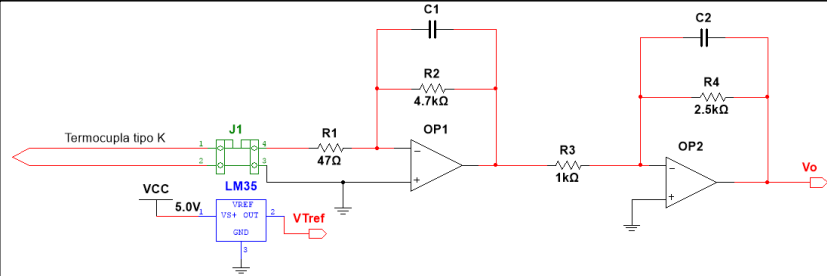
\includegraphics[width=0.8\linewidth]{media/circuito}
	\caption{Circuito amplificador de termocupla}
	\label{fig:circuito}
\end{figure}

En el figura \ref{fig:circuito} se muestra el amplificador de voltaje generado por diferencia temperatura en el conductor de la termocupla, siendo así que este circuito además de amplificar incluye el filtrado de la señal para una frecuencia de corte 6Hz definida por los capacitores $C_1$ y $C_2$ además de agregar una ganancia definida por la configuración de resistencias de $R_1$ a $R_4$.

La ganancia total del circuito esta definida por el producto de la ganancia individual de cada Amp. operacional o bloque elevando así el nivel de voltaje CD obtenido en la salida, por tanto para determinar A (ganancia) se consideraran operacionales ideales y se realizará un calculo independiente para facilitar el análisis matemático detallando al mismo tiempo que cada operacional tiene una configuración inversora amplificando negativamente por etapa permitiendo así que este factor de incremento se haga positivo.

En las ecuaciones se puede apreciar el proceso detallado para cada elemento definiendo una capacitancia $C_1 = $ y $C_2 = $ para obtener la ganancia deseada, así mismo se puede además obtener una diagrama de bode para realizar el análisis en frecuencia, sin embargo al usar una señal CD de entrada esto no es de vital importancia para el análisis.

\begin{align*}
	Z_1 = R_2 || C_1\\
	Z_1 = \frac{R_2}{1 + SC_1R_2}\\
	Luego \\
	Z_2 = R_4 || C_2\\
	Z_2 = \frac{R_4}{1 + SC_2R_4}\\
\end{align*}

Considerando las expresiones previas se deduce a partir de la configuración en los operaciones la formula para su función de transferencia como el bloque de retroalimentación respecto del bloque de entrada, siendo así que se obedece la siguiente expresión $\frac{V_O}{V_i} = \frac{R_F}{R_i} $, aplicando esta relación se obtiene la función de transferencia completa del circuito mediante el uso de $Z_1$ y $Z_2$, obteniendo las expresiones \ref{eq:ft-opam1} y \ref{eq:ft-opam2} para el primer y segundo operacional respectivamente.

\begin{equation}
	\frac{V_y}{V_i} = \frac{R_2}{R_1(1 + SC_1R_2)}
	\label{eq:ft-opam1}
\end{equation}

\begin{equation}
	\frac{V_o}{V_y} = \frac{R_4}{R_3(1 + SC_2R_4)}
	\label{eq:ft-opam2}
\end{equation}

La ganancia total se obtiene a partir del producto de ambos resultados estableciendo así una función de transferencia de un sistema de 2do orden, sin embargo en este mismo para poder obtener una expresión para la ganancia de forma certera es necesario correlacionar el resultado obtenido con la expresión general de un sistema de 2do orden \cite{ogata_ingenieria_control_moderna}, mostrado en la ecuación \ref{eq:sistema-2do-orden}

\begin{equation}
	H(S) = \frac{K\omega_n}{S^2 + 2\xi\omega_nS +  \omega^2_n} 
	\label{eq:sistema-2do-orden}
\end{equation}

Con esta consideración la función de transferencia del circuito resulta como en \ref{eq:ft-circuito}

\begin{equation}
	%\frac{V_o}{V_i} = \frac{ \frac{R_2R_4}{R_1R_3C_1C_2R_2R_4} }{ S^2 + S\frac{C_1R_2 + C_2R_4}{C_1C_2R_2R_4} + \frac{1}{C_1C_2R_2R_4} } 
	\frac{V_o}{V_i} = \frac{ \dfrac{R_2R_4}{R_1R_3C_1C_2R_2R_4} }{ s^2 +s\frac{C_1R_2 + C_2R_4}{C_1C_2R_2R_4} + \frac{1}{C_1C_2R_2R_4} }
	\label{eq:ft-circuito}
\end{equation}

En la cual mediante la comparación se obtiene que el factor K es equivalente a una relación entre las respectivas resistencias para cada etapa del circuito de la siguiente forma \ref{eq:ganancia}

\begin{equation}
	K = \frac{R_2R_4}{R_1R_3}
	\label{eq:ganancia}
\end{equation}

Siendo así que al utilizar los valores definidos en la figura \ref{fig:circuito} desde $R_1$ a $R_4$ se obtienen un $K = 250$, siendo este un valor considerable para voltajes de entrada elevados, sin embargo que es muy adecuado para valores en la escala de los mV \textit{para no saturar las amp. operacionales}.
















